% v2-acmtog-sample.tex, dated March 7 2012
% This is a sample file for ACM Transactions on Graphics
%
% Compilation using 'acmtog.cls' - version 1.2 (March 2012), Aptara Inc.
% (c) 2010 Association for Computing Machinery (ACM)
%
% Questions/Suggestions/Feedback should be addressed to => "acmtexsupport@aptaracorp.com".
% Users can also go through the FAQs available on the journal's submission webpage.
%
% Steps to compile: latex, bibtex, latex latex
%
% For tracking purposes => this is v1.2 - March 2012
\documentclass{sig-alternate} % V1.2

%\acmVolume{VV}
%\acmNumber{N}
%\acmYear{YYYY}
%\acmMonth{Month}
%\acmArticleNum{XXX}
%\acmdoi{10.1145/XXXXXXX.YYYYYYY}
\usepackage{graphicx}
\usepackage{gnuplottex}
\usepackage{tikz}
%\usepackage[T2A]{fontenc} 
%\usepackage[utf8]{inputenc}
\usepackage{graphicx}
%\usepackage{indentfirst}
\usepackage{hyperref}
\usepackage{textcomp}

\begin{document}

\makeatletter
\def\@copyrightspace{\relax}
\makeatother

\title{Generalized LL parsing for context-free constrained path search problem}

\sloppy

\numberofauthors{2}

\author{
\alignauthor
       Semyon Grigorev\\
       \affaddr{Saint Petersburg State University}\\
       \affaddr{7/9 Universitetskaya nab.}\\
       \affaddr{St. Petersburg, 199034 Russia}\\
       \email{semen.grigorev@jetbrains.com}
\alignauthor
       Anastasiya Ragozina\\
       \affaddr{Saint Petersburg State University}\\
       \affaddr{7/9 Universitetskaya nab.}\\
       \affaddr{St. Petersburg, 199034 Russia}\\
       \email{ragozina.anastasiya@gmail.com}
}

\maketitle

\begin{abstract}
Aaaabstract is very abstract....

\end{abstract}

\section{Introduction}
Graph data model and graph data bases are very popular in many different areas such as bioinformatic, semantic web, social networks etc.
Extraction of paths satisfying specific constraints may be useful for graph structured data investigation and for relations between data items detection.
Path querying with constrains formulated in terms of formal grammars is a specific problem named formal language constrained path problem~\cite{FLCpathProblem} and research in this area is still actual~\cite{DirOfBigGraphAnalysis}.

Query result exploration is a challenge~\cite{hofman2015separabilityForRegQueryDebugging}. Our approach can be helpful.

Graph parsing may be required in different areas: formal verification, string-embedded language processing, graph data bases quering.

String-embedde languages.
Regular approximation for value set of string variable.
In orded to check corectness or safety (sql injections)... all generated strings (all paths from start states to final states) are correct w.r.t some context-free grammar.
For example grammar of one of SQL dialects.
GLR-based for string-embedded SQL checking~\cite{Alvor1, Alvor2}.
Solution based on RNGLR~\cite{rnglr} for relaxed parsing of string-embedded languages~\cite{relaxedRNGLR} which allow to find all path between two specified vertices.

\section{Generalized LL parsing Algorithm}

GLL is generalized top-down parsing algorithm which handle all context-free grammars (including left recursive) with worst-case cubic time complexity and linear for LL grammars.

Grammar slot is a: 

GLL use descriptors

Descriptor: a triple $(L, s, j)$ where $L$ is a line label, $s$ is a stack and $j$ is a position in the input.

allows to restore parsing

Graph structured stack (GSS)~\cite{Tomita} for multiple stack combining to prevent duplication.
In GLL each GSS node is pair of position in input and grammmar slot.

\subsection{Shared pached parse forest}

Shared Packed Parse Forest (SPPF) is a spectial data structure for derivation forest compact representation. 
Binarized form of SPPF proposed in~\cite{brnglr} and it allow to achive worst-case cubic space complexity.

Let we present an example of SPPF for ambiguos grammar $G_0$ (pic~\ref{grammarG0}).

\begin{figure}[h]
   \begin{center}
\begin{verbatim}
   0: s = NUM
   1: s = LBR s RBR
   2: s = s s
\end{verbatim}
   \caption{Grammar $G_0$}
   \label{grammarG0}        
   \end{center}
\end{figure}

Here \verb|N| is token for number, \verb|L| and \verb|R| are tokens for '(' and ')'  respectively.

Let we parse the sentence \verb|(1)(2)(3)|. There are two diferent lefmost derivations of this sentence in grammar $G_0$ ($\rightarrow ^ n$ denote an application of production with nimber $n$): 
\begin{enumerate} 
    \item $s \rightarrow ^ 2 s s \rightarrow ^ 2 s s s \rightarrow ^ 1 L s R s s \rightarrow ^ 0 L N R s s \rightarrow ^ 1 
    L N R L s R s \rightarrow ^ 1 L N R L s R s \rightarrow ^ 0 L N R L N R s \rightarrow ^ 1 L N R L N R L s R \rightarrow ^ 0 L N R L N R L N R$
    \item $s \rightarrow ^ 2 s s \rightarrow ^ 1 L s R s  \rightarrow ^ 0 L N R s \rightarrow ^ 2 L N R s s  \rightarrow ^ 1 
    L N R L s R s \rightarrow ^ 1 L N R L s R s \rightarrow ^ 0 L N R L N R s \rightarrow ^ 1 L N R L N R L s R \rightarrow ^ 0 L N R L N R L N R$
\end{enumerate}
    , SPPF should contains two trees. SPPF presented in figure~\ref{sppfSample} will be constructed.


\begin{figure}[h]
    \begin{center}
        \includegraphics[width=8cm]{dot/Brackets.pdf}
        \caption{SPPF}
        \label{sppfSample}        
    \end{center}
\end{figure}

Binarised SPPF is a graph where !!! and each node has one of four types and one node marked as 'root' --- node for start nonterminal.

\begin{itemize}
    \item terminal node
    \item nonterminal node
    \item intermidiate node
    \item ....
\end{itemize}

Further we will remove redudant nodes from SPPF to simplify it and decrease size of structure.

GLL can use SPPF~\cite{gllParsingTree} for results representation achive cubic space complexity with binarised version.


\section{Preliminaries}

Let we introduce some definitions.
\begin{itemize}
  \item Context-free grammar $G=(N, \Sigma, P, S)$ where $N$ is a set of nonterminal symbols, $\Sigma$ is a set of nonterminal symbols, $S \in N$ is a start nionterminal, and $P$ is a productions set. 
  \item Directed graph $M = (V,E,L)$ where $V$ --- vertices set, $L \subseteq \Sigma$ --- edge labels set, $E\subseteq V\times L\times V$. 
  We assume that there are no parallel edges with equal labebs: for every $e_1=(v_1,l_1,v_2) \in E, e_2=(u_1,l_2,u_2) \in E$ if $v_1 = u_1$ and $v_2 = u_2$ then $l_1 \neq l_2$.
  \item Helper function for edge's tag calculation $tag: E \rightarrow L; tag(e = (v_1,l,v_2), e \in E) = l$.
  \item Concatenation operation $\oplus: L^+ \times L^+ \rightarrow L^+$.
  \item Path $p$ in graph $M$. \\ $p = (v_0,l_0,v_1),(v_1,l_1,v_2),\dots,(v_{n-1},l_{n-1},v_n) = e_0,e_1,\dots,e_{n-1}$ where $v_i \in V$,$e_i \in E$, $l_i \in L$, $|p| = n \leq 1$. 
  \item Set of paths $P = \{p: p \text{ path in } M\}$
  \item Helper function for string produced by path calculation $\Omega: P \rightarrow L^+$.\\ $\Omega(p = e_0,e_1,\dots,e_{n-1}, p \in P) = tag (e_0) \oplus \dots \oplus tag (e_{n-1})$.
\end{itemize}

As a result we can define that context-free language constrained path querying meens that each path $p = e_0,\dots,e_{n-1}$ from result set satisfied with next constraint: $\Omega(p) \in L(G)$. 

As a motivation of context-free constraints importance let we introduce the next example.
Let we have graph $M=(\{0;1;2;3\},E,\{A;B\})$ presented in figure~\ref{input} where labels represent $parent (A)$ and $child (B)$ relations. 
Suppose for each $n \leq 1$ we want to find all $n$-th generation descendants with a common ancestor.
In the other worlds, we wath to find all paths $p$, such that $\Omega(p) \in \{AB; AABB; AAABBB; \dots\}$ or $\Omega(p) = A^n B^n$ where $n \geq 1$.
This constraint can not be specified with regular language as far as $L=\{A^n B^n; n \geq 1\}$ is not regular but context free.
Required language can be specified by grammar $G_1$ presented in picture~\ref{grammarG} where $N = \{s; middle\}$, $\Sigma = \{A; B\}$, and $S = s$.

\begin{figure}[h]
    \begin{center}
        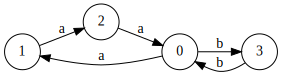
\includegraphics[width=6cm]{dot/input.pdf}
        \caption{Input graph $M$}
        \label{input}        
    \end{center}
\end{figure}

\begin{figure}[h]
   \begin{center}
\begin{verbatim}
   0: s = L s R 
   1: s = middle
   2: middle = L R
\end{verbatim}
   \caption{Grammar $G_1$ for language $L=\{L^n R^n; n \geq 1\}$}
   \label{grammarG}        
   \end{center}
\end{figure}

\section{GLL-based graph parsing}
We propose a context-free language constrained path problem solution which allow to find all paths satisfied specified arbitrary context-free grammar and to construct implicit representation of result. 
Finite representation of result set with structure related to specified grammar may be useful not only for results understanding and processing but also for query debugging especially for complex queries. 

Our solution is based on generalized LL (GLL)~\cite{scott2010gll, FastPracticalGLL} parsing algorithm which allow to process ambiguous context-free grammars.
Complexity is $O(n^3)$ in worst case and linear for unambiguous grammars, that better then complexity of CYK and Earley which used as base in other solutions (for example~\cite{ConjCFPathQuery}, ~\cite{GraphQueryWithEarley}).
This fact allow to demonstarte better performance on linear subgraphs and unambiguous grammars.
Also it is not necessary to transform input grammar to CNF which required for CYK.

Basic idea --- let position is vertex in graph. As far as we work with context-free languages it is not important how this descriptor was created. We can merge it. 

We implement some optimizations:~\cite{FastPracticalGLL}

We also use SPPF for result representation.
In our case more then one root may be specified. For example, look at picture!!!! We 

\subsection{Complexity}

Worst case: $O(|V|^3*|E|)$ For unambiguous grammar:$O(|V|*|E|)$


Descriptor: $(L, s, j)$ $|L| = f(G), |j| = |V|, |s| = |GSS.Nodes|$
GSS node $N = (lbl, j), |lbl| = f(G), |j| = |V|$
So $V^2$ descriptors.
For each descriptor we should examine all outgoing edges: $V^2*E$
For all results of previous step we should find internal structures. It is possible in linear time~\cite{modellingGLL}.
So, result is $O(V^3*E)$ in worst case.
$O(|V|*|E|)$ for unambiguous grammar.
$O(|V|^3*l)$ where $l = \frac {\sum\limits_{v \in V} deg^+(v)}{|V|}$
$O(|V|^3*l)$ where $l = \max\limits_{v \in V} deg^+(v)$




\subsection{Example}
In details, main function input is graph $M$, set of start vertices $V_s\subseteq V$, set of final vertices $V_f\subseteq V$, grammar $G_1$.
Output is Shared Packed Parse Forest (SPPF)~\cite{SPPF} --- finite data structure which contains all derivation trees for all paths in $M$, $\Omega(p) \in L(G_1)$ and allows to reconstruct any of paths implicitly.
As far as we can specify sets of start and final vertices, our solution can find all paths in graph, all paths from specified vertex, all paths between specified vertices. 
Also SPPF represents a structure of paths in terms of derivation which allow to get more useful information about result.

Let we introduce the next example. Grammar $G_1$ is a query and we want to find all paths in graph $M$ (presented in picture~\ref{input}) matched this query.
Result SPPF for this input is presented in picture~\ref{SPPF}. Note that presented version does not contein obsolete nodes.

\begin{figure}[h]
    \begin{center}
        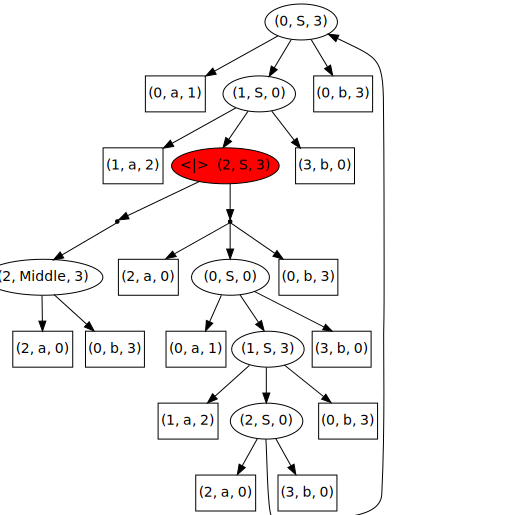
\includegraphics[width=9cm]{dot/AnBn.pdf}
        \caption{Result SPPF for input graph $M$(pic.~\ref{input}) and query $G_1$(pic.~\ref{grammarG})}
        \label{SPPF}        
    \end{center}
\end{figure}

We use next markers for nodes.
\begin{itemize}
    \item Node with rectangle shape labeled with $(v_0, T, v_1)$ is terminal node. 
    Each terminal node corresponds with edge in the input graph: for each node with label $(v_0, T, v_1)$ there is $e\in E: e=(v_0,T,v_1)$.
    Duplication of terminal nodes is only for figure simplification.
    \item Node with oval shape labeled with $(v_0, nt, v_1)$ is nonterminal node. 
    This node denote that there is at least one path $p$ from vertex $v_0$ to vertex $v_1$ in input graph $M$ such that $nt \Rightarrow^*_G \Omega(p)$.
    All paths matched this condition can be extracted from SPPF by left-to-right top-down graph traversal started from respective node. 
    \item Filled node with oval shape labeled with $(<\mkern-11mu | \mkern-11mu> (v_0, nt, v_1))$ is nonterminal node denote that there are more then one path from $v_0$ to $v_1$ such that $nt \Rightarrow^*_G \Omega(p)$.
    \item Node with dot shape is used for representation of derivation variants.
    Subgraph with root in one such node is one variant of derivation.
    Parent of such nodes is always node with label $(<\mkern-9mu | \mkern-9mu> (v_0, nt, v_1))$.
    \item $v_0$ and $v_1$ are left and right extensions of node respectively.
\end{itemize}

As an example of derivation structure usage we can find 'middle' of any path in example above simply by finding corresponded nonterminal $middle$ in SPPF.
So we can found that there is only one common ancestor for all results and it is vertex with $id = 0$. 

Extensions stored in nodes allow to check whether path from $u$ to $v$ exists and extract it. 
Path extraction is SPPF traversal. 
Let for example we want to find path satisfying specified constraints fron vertex $0$.
To do this we should find vertices with label $(0, s, \_)$ in SPPF. There are two vertices: $(0, s, 0)$ and $(0, s , 3)$.
In our example there is cycle in SPPF so there are \textbf{at least} two different paths: $p_0=\{(0,A,1);(1,A,2);(2,A,0);(0,B,3);(3,B,0);(0,B,3)\}$ and $p_1=\{(0,A,1);(1,A,2);(2,A,0);(0,A,1);(1,A,2);(2,A,0);\\ (0,B,3);(3,B,0);(0,B,3);(3,B,0);(0,B,3);(3,B,0)\}$ .

\section{Evaluation}

We perform some experiments on syntatic graphs.
Full graphs and graphs with structure presented in figure !!!.
All paths from all vertices and all paths from one specified vertex. 
For full graph also all paths between two specified vertices.

We use two grammars for balanced brakets in order to investigate performance relations with grammar ambiguity: ambiguos grammar $G_0$~\ref{grammarG0} and unambiguos grammar $G_2$~\ref{grammarG2}.

\begin{figure}[h]
   \begin{center}
\begin{verbatim}
   0: s = L s R s 
   1: s = eps
\end{verbatim}
   \caption{Unambiguos grammar $G_2$ for balanced brackets}
   \label{grammarG2}        
   \end{center}
\end{figure}


All tests were performed on a PC with following characteristics:
\begin{itemize}
\item OS Name: Microsoft Windows 10 Pro
\item System Type: x64-based PC
\item CPU: Intel(R) Core(TM) i7-4790 CPU @ 3.60GHz, 3601 Mhz, 4 Core(s), 4 Logical Processor(s)
\item RAM: 32 GB
\end{itemize}

Results presented in figure~\ref{pic:DoubleCyclesPerf}.
From all and from one vertex is because descriptors reusing.

\begin{figure}[h]
\centering%
\begin{gnuplot}
set terminal epslatex color size 9cm,8cm
set key box top left
set key width 2
set key opaque
set sample 1000
set xlabel '$x$-label'
set ylabel '$y$-label
plot 'perf/1' using 1:2 with lines ls 2 ti '$P_2$',\
     'perf/1' using 1:3 with lines ls 3 ti '$P_2$',\
     'perf/1' using 1:4 with lines ls 4 ti '$P_2$',\
     'perf/1' using 1:5 with lines ls 5 ti '$P_3$'
 \end{gnuplot}
\caption{Performance on C graph for grmmars $G_0$ and $G_2$}%
\label{pic:DoubleCyclesPerf}%
\end{figure}%

To summarise we can say that performance for unambiguos grammars is better then for ambiguos. 

\section{Conclusion and future work}
We propose GLL-based algorithm for context-free path querying which construct finite structural representation of all paths satisfying given constrains.
Provided data structure can be useful for result investigation and processing, and debugging.
Presented algorithm implemented in F\# and available on GitHub:\url{https://github.com/YaccConstructor/YaccConstructor}.

Our future work is evaluation on real dataset and real queries.

Also we are worcing on performance improvement by implementation of recently proposed modifications in original GLL algorithm~\cite{FGLL}.
Generalization of grammar factorization may be useful for regular query processing.

We are working on utilisation of GPGPU and multicore CPU power for graph parsing problem with Valiant~\cite{valiantParsingWithMatrixMultiplication} algorithm modification proposed by Alexander Okhotin~\cite{okhotin2014parsingWithMatrixMultiplication}

\bibliographystyle{abbrv}
\bibliography{ContextFreeConstrainedPathFindingInGraph}

%\bibitem{PathQuerySemantic}
%Hellings, J. (2015). Querying for Paths in Graphs using Context-Free Path Queries. arXiv preprint 
%arXiv:1502.02242.

%\bibitem{CFPathQuery}
%Sevon, P., /& Eronen, L. (2008). Subgraph queries by context-free grammars. Journal of Integrative 
%Bioinformatics, 5(2), 100.


\end{document}
